\chapter{Sample characterization}

\section{Optical setup}

\begin{figure}
	\centering
	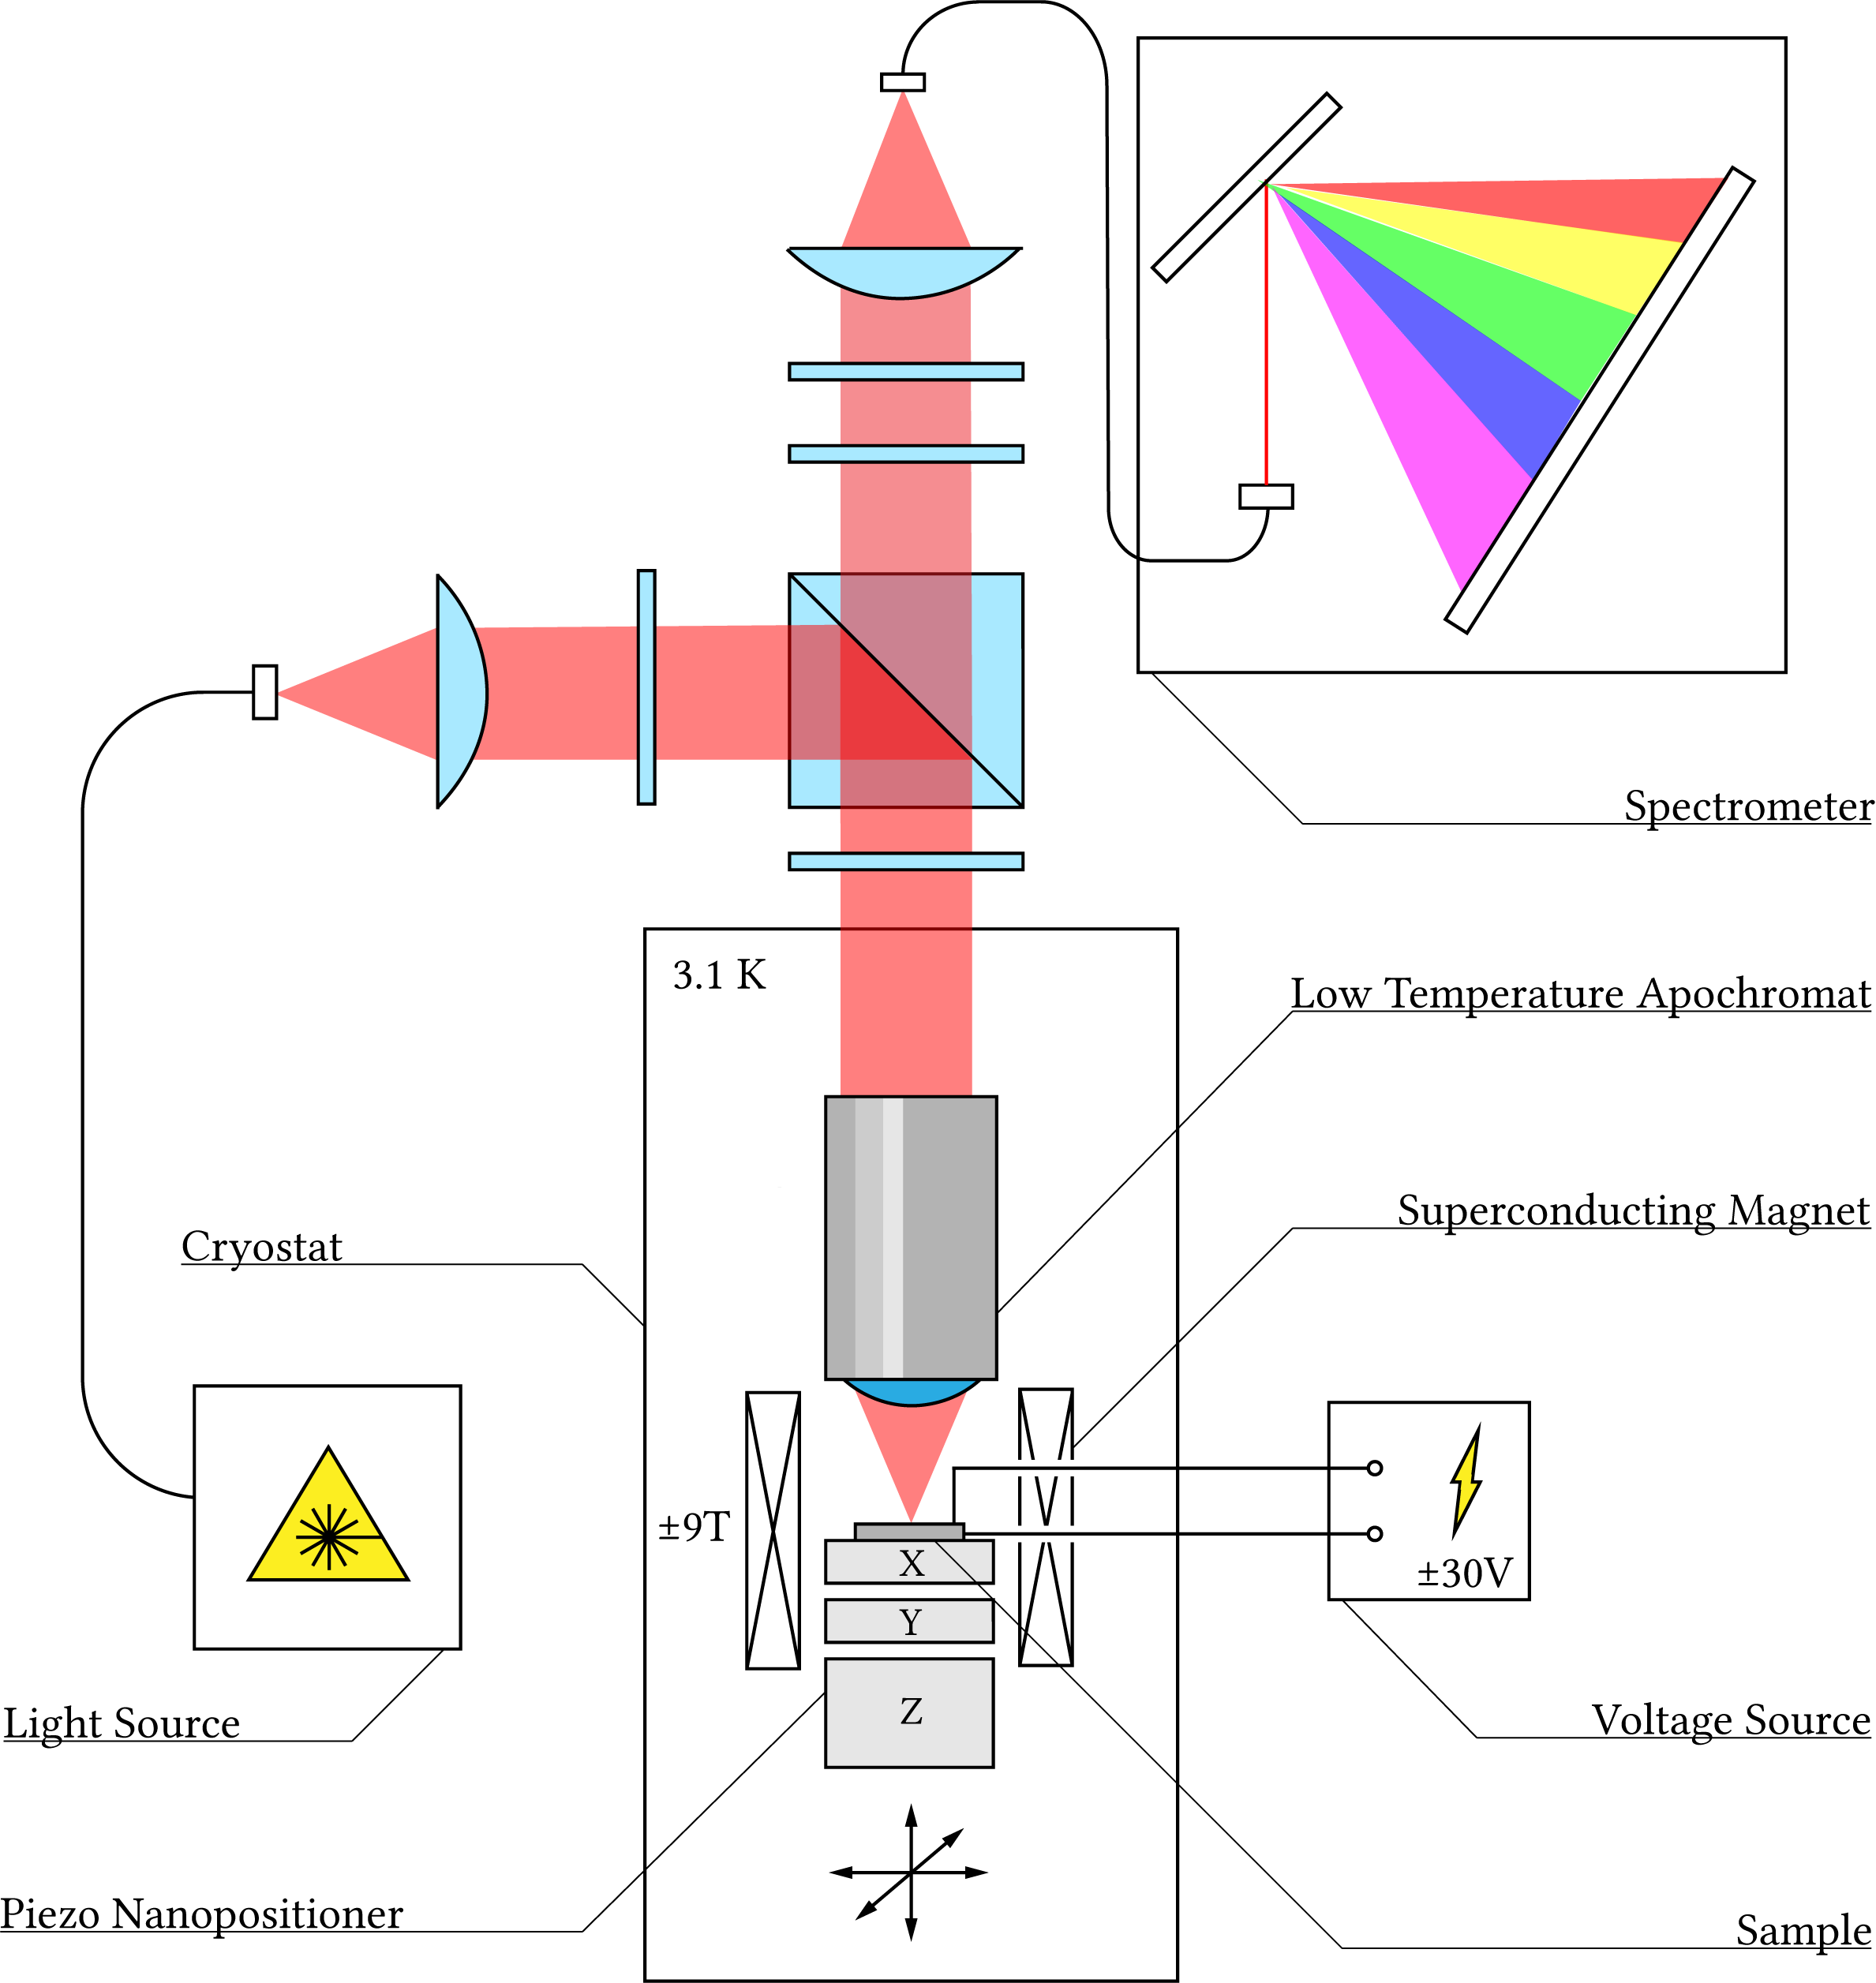
\includegraphics[width=.8\textwidth]{OptischerAufbau.png}
	\caption{Optical setup for confocal spectroscopy: Light from a \textbf{laser}-source is guided to the setup in a single mode opical fibre and collimated. To cut off raman-modes, that are created in the fibre a \textbf{shortpass} filter is installed behind the collimator. A \textbf{linear polarizer} defines a polarization axis. A \textbf{beam-sampler} is reflecting the excitation beam into a \textbf{low temperature apochromat}, whose focus lies on the sample, with a spotsize of \textasciitilde\- 0.5\mu m. The sample is mounted on a \textbf{piezo nanopositioner}, that is placed inside a \textbf{cryostat} at a temperature of up to 3.1 K or in a container of liquid helium at 4.2 K. The cryostat is equipped with a \textbf{superconducting magnet} that can supply a homogenious magnetic field up to 9T. The sample electrodes are connected to a \textbf{voltage source} (Yokogawa) that supplies {\small$\pm$}32V. The detection spot is identical with the excitation. The reflection or photoluminescence is collimated again in the objective and passes through a \sigma$^+$/\sigma$^-$-analyzer consisting of a \textbf{quarter waveplate} and a \textbf{linear polarizer}, before being focussed in the detection fibre that connects to a \textbf{spectrometer}. A \textbf{camera} can be used to monitor the spot and image the sample, if it is brought out of focus.}
	\label{opticalsetup}
\end{figure}

The optical setup is a confocal microscope. In contrast to a ``conventional'' microscope, the sample is placed in the focal plane of a low temperature objective. The focal point is the same for excitation of the sample and the detection of the reflection or photoluminescence signal, hence the name. A scheme of the complete setup can be seen in Figure \ref{opticalsetup}. The excitation beam from a laser is guided to the so called excitation arm with a single mode optical fibre. It passes though a linear plolarizer to define a polarization axis and is reflected to the objective by a beam-sampler. To analyze the mostly circularly polarized light of the detection beam, it passes through a quarter waveplate and another linear polarizer and is focussed into another optical fibre, that is connected to a spectrometer. The sample is mounted on a piezo nanopositioner inside a cryostat or can of liquid helium and connected to a voltage source, to tune the charge density in the \tmdg flake. A strong, homogenious magnetic field can be supplied by a superconducting magnet.

For photoluminescence spectroscopy, the sample is excited with a laserbeam with a narrow frequency profile and a higher intensity. Because this beam has a much higher intensity, than the collected \textsc{pl} it is tuned to a higher frequency than the main exiton resonance. A shortpass filter in the excitation arm makes sure, no raman modes from the optical fibre pollute the spectrum. A longpass filter, right before the optical fibre of the detection arm blocks the laser, so that only \textsc{pl} reaches the spectrometer. To optain a reflection spectrum, these filters are omitted. Instead, the sample is illuminated with a broad band light source at a low power. To find the signal, a background spectrum, recorded in absence of the \tmdg flake is substracted from the main spectrum.

\[ 
	S_R = \frac{\Delta R}{R} = \frac{R_{\mathrm{flake}} - R_{\mathrm{background}}}{R_{\mathrm{background}}}
\]

The signal $S_R$ is the difference of the Reflection signals of \tmdg flake and background. The devision by the background reflection is made to normalize the signal. The resulting reflection spectrum should show only features, of the flake. In practice, the obtained data has to be evaluated with some precautions in mind, to avoid misidentifiying for example interference effects due to differences in \hbng thickness as features of the absorption behaviour of the sample.

\section{Sample characterization}

There are two dimensions to characterize the quality of a sample. Its optical properties must include narrow linewidths, to identify different features of the spectrum and it has to be gate-tunable, which means the contact of \tmdg flake to the electrode as well as the backgate have to function and the \sio layer has to sustain enough voltage to tune in and out of neutral and charged regimes.

\section{Electrical characterization}

To function of a gate-tunable \tmd-device is threefold. The top-gate electrode has to be in contact with the flake of interest, the contacts to the backgate have to function, especially at low temperature and the dielectric has to hold enough voltage to see effects in the optical spectrum. Because the flake has only one contact, no transport measurement is possible. Hence the quality of the top-gate contact can only be assessed by seing its effects in the optical spectrum. The other two criteria can be checked and quantified without any optical means. As mentioned in (Section vong 1 fabrikation) the p-doped silicon bulk material, that is used as the back-gate electrode is prepared with two contacts. Both of these contacts can be connected to a simple multimeter, to measure the resistance between them. For this particular material a resistance of 5-6 \Omega\ means, the contacts function as planned. If there is no contact or a high resistance, one of the contacts might still be functional. This can be assessed by observing the spectrum for different voltages, just like the top-gate. Nevertheless, having an additional check by using two back-gate contacts, helps troubleshooting in case of issues with the device.

The quality of the dielectric is quantified by measuring the capacity of the device for different voltages and monitoring the leak current (see Figure CV). A constant voltage across the desired range of operation ({\small$\pm $}30V) is added to a small alternating current of small amplitude ($U_0 = $ 10 mV$_{pp}$, $f = $ 77.1 Hz). The real part of the resulting current is the resistive current, or leakage and the imaginary part is proportional to the capacity. Both parts can be measured in a lock-in amplifier. For our devices, the leakage current at low voltages should not exceed the pico-ampere range. For characterizing the dielectric the constant voltage can be raised until the resistive current starts rising exponentially. The corresponding voltage is the maximum, that should be applied in the particular sample, because a higher voltage can result in charges breaking through the dielectric and forming conducting chanels, thus disabling the gate-tunability permanently. This sensitivity is the reason to use this more complicated characterization method instead of simply monitoring the current while applying voltages directly. Because very low currents can be measured with the lock-in amplifier, the boundary of safe operation can be approached very carefully.

%Here is a figure of CV-measurement

\section{Spectral resolution}
\subsection{Spectral features at different doping levels}

\begin{figure}
	\begin{subfigure}{0.49\textwidth}
		\caption{}
		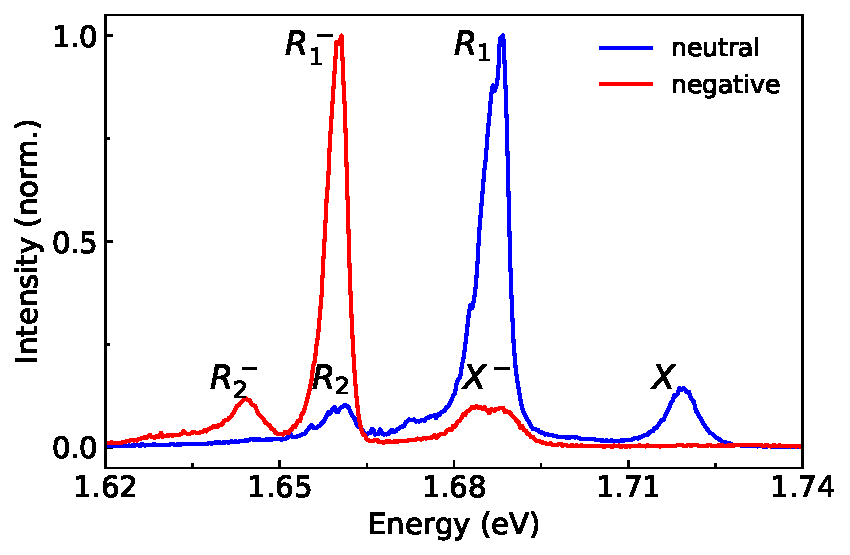
\includegraphics[height=0.65\textwidth]{spectrum_neutral_negative}
	\end{subfigure}
	\begin{subfigure}{0.49\textwidth}
		\caption{}
		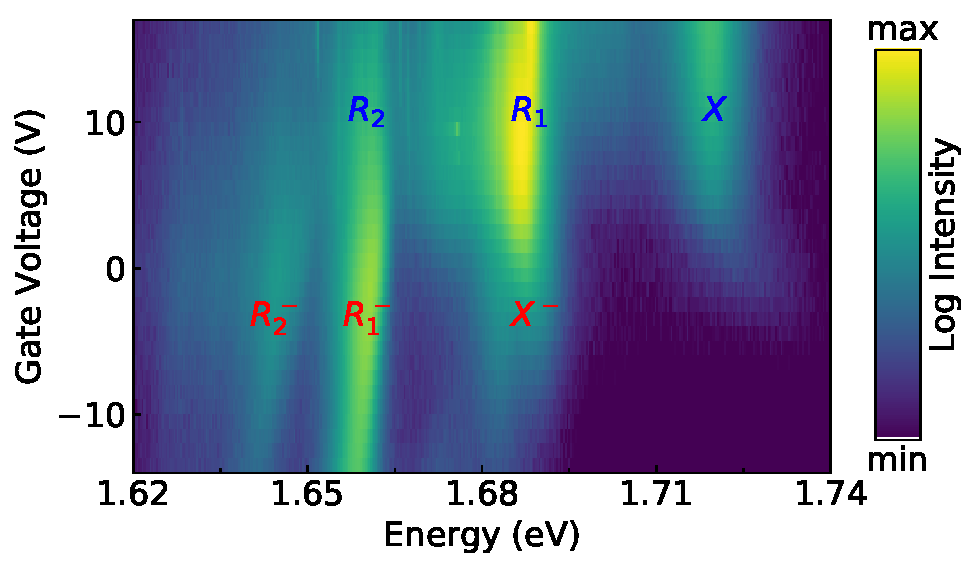
\includegraphics[height=0.65\textwidth]{Voltsweep}
	\end{subfigure}
\end{figure}

%\subsection{Measuring the valley zeeman effect}